\chapter[\hspace{0pt}绪\hskip\ccwd{}论]{{\heiti\zihao{3}\hspace{0pt}绪\hskip\ccwd{}论}}
\label{ch:introduction}

\section[\hspace{-2pt}研究背景与意义]{{\heiti\zihao{-3} \hspace{-8pt}研究背景与意义}}
\label{sec:intro-background}

近年来,深度学习(Deep Learning)的迅猛发展引发了人工智能领域的范式转变。基于多层神经网络的大规模模型在图像识别、语音识别、自然语言处理等任务上取得了前所未有的突破。从2012年AlexNet掀起深度学习热潮以来,研究者不断通过加深网络深度、增大模型参数规模以及利用更庞大的训练数据来提升模型性能。例如,2019年问世的GPT-2模型拥有约15亿参数,而2023年发布的GPT-4模型规模已达到惊人的1万亿参数[1]。模型规模和数据量的指数级增长极大地提高了AI系统的表现力,但也带来了对计算资源近乎“贪得无厌”的需求[1]。OpenAI的统计显示,自2012年以来用于训练顶尖AI模型的计算量增加了超过30万倍,训练所需计算量大约每3.4个月就翻一番[1]。这一趋势表明,通过大规模化换取性能提升的做法正推动计算需求呈爆炸式增长。然而,如此依赖规模扩张的范式也埋下了隐忧:当模型性能与资源投入形成正相关时,“性能—资源”之间的矛盾日益凸显。

首先,深度模型规模化带来的性能与资源矛盾已经成为当前AI研究的重要挑战。一方面,经验表明更大的模型和更多的数据通常能带来更优的效果,推动着诸如BERT、GPT等“基础模型(Foundation Model)”不断朝更高参数量发展。更大的模型展现出前所未有的复杂推理和认知能力,例如在语言对话、代码生成等任务上涌现出小模型无法具备的新能力。这些现象印证了所谓“规模定律”(Scaling Law),即模型性能可以通过扩大参数和数据规模持续提升。然而另一方面,模型性能的提升以巨大的资源消耗为代价:需要海量标注数据来训练,需要成百上千的GPU/TPU算力来迭代更新参数,并消耗惊人的电能与时间。例如,OpenAI的分析指出,2012年至2018年间深度学习模型训练的计算量累计增长了约30万倍[2]。这样的计算需求远远超出了摩尔定律的增长速度,导致硬件升级难以追赶模型膨胀的步伐[3]。当今最顶尖的模型训练往往要消耗数百万美元的计算成本,只有极少数科技公司和研究机构具备这样的算力投入。这种资源高度集中现象使得学术界和中小企业难以参与同等规模的模型研究,深度学习研究在某种程度上正变成“资源军备竞赛”。

更为严峻的是,在大模型背后所隐藏的数据与能耗问题同样不容忽视。数据方面,监督深度学习的成功极大依赖于大规模标注数据集。然而对于许多垂直领域和长尾任务来说,获取海量高质量标注数据并不现实。例如在医疗影像、遥感识别等领域,标注一个大型数据集往往代价高昂且耗时费力。大模型在ImageNet、WebText等通用数据上取得的成功,难以直接复制到这些数据匮乏的场景中。这就导致数据制约了模型性能:没有足够的数据支撑,再庞大的模型也难以充分训练而表现出色。能耗方面,训练和部署深度模型的能源消耗迅速攀升,引发了对AI环境影响的担忧。有研究估计,单次训练一个大型Transformer语言模型可能产生高达 284吨二氧化碳 的碳排放[4](相当于几十辆汽车一年的排放量),凸显出当前AI模型“高碳足迹”的问题[5][4]。这种巨大的能耗需求不仅带来环境代价,也使得模型训练的经济成本攀升。Strubell等人的研究曾指出,训练一个前沿NLP模型的耗电量相当于五辆汽车的全生命周期能耗[2]。在能源价格上涨和碳中和目标的双重压力下,如何控制AI模型的能耗已成为AI可持续发展必须面对的问题。

上述性能与资源的矛盾为学术界和工业界敲响了警钟:过去那种简单依赖“堆数据、堆算力、堆参数”获取更高性能的范式难以长期维系。一方面,硬件供应链已经出现瓶颈,高端GPU往往供不应求且价格高企;另一方面,社会各界开始呼吁AI研究应关注能效比,倡导“绿色AI(Green AI)”理念,将计算成本和能源消耗纳入科研评价指标[6]。Green AI的倡议者指出,深度学习的计算开销正成为学术研究的门槛,令资源不足的高校和发展中国家的研究者难以参与其中[6]。因此,他们主张在发表研究成果时,不仅报告模型精度,还应报告训练所需的计算量和财务成本,以推动更高效的方法涌现[7]。正如Schwartz等人在“Green AI”论述中所言,如果不将效率纳入考量,深度学习研究将沦为“只有少数拥有最深口袋者才能玩的游戏”[6]。为了让AI研究“更绿色且更包容”,学术界开始重视效率导向的评价:例如每正确分类一张图像所需的能耗、达到一定准确率所需的样本数量、每提升1\%性能所需的额外算力等指标。这些努力的目标是促使AI技术朝着高效、可持续的方向发展,使得哪怕是只有一台笔记本电脑的普通学生也有机会从事高质量的深度学习研究[7]。

基于上述背景,如何在有限资源条件下高效构建深度模型已经成为亟待解决的核心科学问题。所谓高效构建,指的是在满足低标注数据、低计算开销、低能耗等多重约束的前提下,最大化模型的性能产出。具体而言,研究者希望在有限标注数据下训练出高精度的模型(提升数据效率),在有限算力/评估预算下迅速找到优良的模型结构(提升搜索效率),以及在有限训练时间和能耗下获得满足任务需求的模型(提升训练效率)。这一目标反映出与传统深度学习范式的转变:过去我们关注的是“性能最大化”,而现在必须在性能与资源之间找到最佳折中,用单位资源获取尽可能多的性能。高效深度模型构建的意义不仅在于技术指标的提升,更在于它将决定AI技术未来发展的普惠性和可持续性:

\begin{itemize}
	\item 数据效率(Data Efficiency):提升数据效率意味着模型在少样本、弱标注的情况下依然具备良好的泛化性能。这对许多现实场景至关重要,如医疗诊断中的罕见病识别、工业质检中的瑕疵检测、自然语言处理中的低资源语言分析等。在这些场景中,标注数据极其有限。如果能大幅降低模型对大规模人工标注的依赖,将使深度学习在更多领域落地成为可能。
	\item 计算/搜索效率(Compute/Search Efficiency):提升搜索效率旨在降低设计和选型优质模型所需的计算代价。这涉及神经网络架构搜索(NAS)等自动化设计方法的高效化。传统NAS往往需要训练并评估成千上万种模型结构,因此计算开销惊人。例如,早期Zoph等人基于强化学习的NAS在CIFAR-10数据集上找到优化架构耗费了800块GPU持续运行28天[8]。如此高昂的成本令普通研究者无法问津。而近年一些高效NAS方法通过性能预测、权重共享等策略,将搜索时间从数百GPU天缩短到数个GPU小时[9]。有研究甚至利用跨领域的预测模型将NAS开销降低到0.1个GPU天,在极短时间内就在ImageNet上找到了Top-1精度76.9\%的优质架构[10]。这证明了通过高效搜索策略,自动设计模型的计算成本能够被大幅削减,为资源受限的团队也能使用NAS打开了大门。
	\item 训练效率(Training/Energy Efficiency):提升训练效率意味着用更少的计算量和能耗完成模型的训练或适应。在传统范式中,训练一个模型往往意味着从随机初始化开始,使用大量算力迭代优化直至收敛。然而在“预训练-微调”时代,已经体现出利用已有模型参数可以显著减少训练所需时间和数据量。例如,将预训练模型Fine-tune到下游任务,比从头训练可节省数量级的计算。更进一步的思路是模型融合:直接将多个已训练模型的参数加以合并,生成一个无需从零训练的新模型。最近的研究表明,通过适当的方法,直接平均或插值不同任务的模型权重也能得到性能优异的多任务模型[11]。这被称为“模型合并”技术,包括模型汤(Model Soup)[12]、球面线性插值(SLERP)、任务向量算术(Task Arithmetic)、TIES融合、DARE预处理等多种方法[11]。模型合并提供了一条不同于传统训练的新径:我们可以将多个任务各自的训练成果通过算术操作合成为单一模型,从而避免了联合训练的高成本。NVIDIA的技术报告指出,通过Model Soup、SLERP、Task Arithmetic、TIES-Merging、DARE等技术,研究者能够有效地合并同系列的多个模型,将不同实验的成果加以复用[11]。与从头多任务训练相比,这种后融合策略几乎不增加新的算力开销,却能获得兼具多项能力的模型[13]。模型融合的成功案例凸显了训练范式的转变:未来很可能“训练”不再意味着完全的参数优化过程,而更多是对已有知识的整合复用,从而大幅节省能耗与时间。
\end{itemize}

综上所述,在有限标签、有限算力、有限能耗约束下追求深度模型的高性能,已成为AI领域的重要命题。解决这一命题不仅有重大的学术价值,更具有深远的实际意义。在学术层面,上述三类效率目标分别对应机器学习的不同研究方向,如小样本学习、自动机器学习、模型压缩与加速等。然而以往这些方向往往各自为战,缺乏统一的框架。本研究试图提出多层次知识迁移这一崭新的整体思路,将上述三方面目标置于同一理论体系下加以考量:即通过知识的迁移复用来同时缓解数据匮乏、算力不足、训练耗时的问题。具体而言,我们将“可重用的先验”细分为三类不同层次:知识层、结构层和参数层,并分别利用它们来提升数据效率、搜索效率和训练效率。

首先,知识层迁移侧重于任务知识的复用。这里的“知识”主要指模型的输出分布和中间表征所包含的关于任务的软信息。例如,在少样本情境下,可以借助预先训练好的教师模型来为训练样本提供更丰富的监督信号(如软标签、特征表示、关联关系等),以指导学生模型学习[14][15]。这种做法被称为知识蒸馏(Knowledge Distillation)[15]。早在Hinton等人提出软目标蒸馏时,就证明了大模型的软概率输出包含丰富的暗知识,可用于提升小模型的性能和泛化。此后,研究者又发展出特征蒸馏、关系蒸馏、自蒸馏等多种变体,使学生模型不仅学习教师的输出分布,还对齐教师的中间激活模式、样本间距离结构乃至相似度关系[16][14]。最近,对比蒸馏等新方法兴起,将对比学习融入知识迁移,通过拉近教师–学生的表示并拉开与负样本的距离来增强蒸馏效果[17]。尤其是在大型预训练模型涌现的背景下(如CLIP、GPT等),对比蒸馏等方法被证明对少样本场景极为有效[17]。总的来说,知识层迁移旨在回答:“当标注数据匮乏时,如何利用已有模型的知识来以较少的样本达到尽可能高的性能?” 其意义在于,充分挖掘大模型中蕴含的先验,使小模型在数据稀缺的条件下站在“巨人的肩膀”上起步。例如,在医疗诊断应用中,可用通用模型的知识来扩充少量标注病例的信息,从而训练出准确率更高的学生模型,这将大大缓解高质量医疗数据不足的问题。

其次,结构层迁移关注网络结构经验的复用,目标是提升模型设计和搜索的效率。深度模型的性能很大程度上取决于其结构设计,但人工设计网络架构既耗时又需要专家经验。神经架构搜索(NAS)通过自动化探索网络拓扑,解放了人工设计,但其高昂的计算代价一直饱受诟病[8]。结构层迁移试图通过迁移先前搜索得到的架构知识,来减少在新任务上重新搜索所需的评估次数和算力投入。比如,可以将源域中表现优秀的网络结构(或其一部分,如卷积单元/细胞结构)迁移为目标任务的搜索起点,缩小搜索范围,从而更快找到优解。此外,近年来的研究引入了架构性能预测模型(Predictor),即用一个学习到的代理模型快速预估给定架构在某任务上的准确率[18]。如果我们已经在某些小型搜索空间上收集了大量架构的性能数据,就可以训练一个性能预测器,并迁移泛化到更复杂的搜索空间中[19][10]。例如,有研究成功地将NAS-Bench-101这样的基准数据上的经验迁移到ImageNet级别的空间中,显著降低了评估开销[10]。另一种结构迁移思路是跨任务或跨空间的架构表示映射。不同任务/数据集往往偏好不同的架构,但它们可能存在某种共性设计原则。通过学习一个统一的架构表示或潜在空间,使源域和目标域的网络拓扑可以直接比较和转换,源域的优良架构就能“翻译”到目标域供进一步优化。这正是本研究中“结构层迁移”要解决的问题:如何定义和学习一种架构表示,使得跨任务的结构知识可以共享,从而在目标任务上快速定位优质架构。结构层迁移的意义在工业界同样突出。例如,在移动端应用中,需要为新出现的应用场景设计高效的轻量模型。如果能够复用先前在类似任务上搜索出的网络模块或拓扑经验,将大幅缩短开发周期,减少反复调优的计算资源浪费。总之,结构层的目标就是回答:“当算力/评估预算有限时,如何利用已有架构经验来以更少的尝试找到性能尽可能好的模型?”

最后,参数层迁移聚焦于模型参数的复用和融合,其直接目标是提升训练效率甚至实现零训练。传统的迁移学习通常指将预训练模型参数作为初始点,在新任务上进行微调。这固然比随机初始化高效得多,但仍需要针对每个新任务执行梯度训练。而参数层迁移试图走得更远:当有多个相关任务各自的模型可用时,能否不经过梯度训练,仅通过参数组合来生成适应新任务的模型?近期涌现的一系列工作表明,这是可能的。例如,Wortsman等提出的模型汤(Model Soup)方法,简单地对多个微调模型的参数取平均,就获得了比单一模型更优的效果[12]。后续研究进一步引入了更精细的参数融合策略,如任务算术(Task Arithmetic)将每个任务的模型差分视为一个“任务向量”,通过加减这些向量来组合出新功能[20];TIES算法则通过“三步走”(裁剪重要权重、选定符号、分段平均)来解决不同模型参数更新之间的冲突[21];DARE方法从另一个角度出发,随机丢弃并缩放各模型的差分参数,以去除冗余和降低不相容性[22]。这些方法的共同点在于:充分利用了现有多个模型的“知识因子”,通过巧妙的数学操作将它们融合成一个模型,相当于在参数空间中进行一次迁移优化。这种做法带来的效率提升是显著的——相比从头训练一个多任务模型,参数融合相当于一个快捷“捷径”。正如NVIDIA技术博客所总结的,模型合并能够最大化多个已定制模型的价值,减少重复训练的浪费,成为联合训练的廉价替代方案[11]。参数层迁移的意义不仅在于节省算力和能耗,更在于提供了一种模型开发的新范式。在实际应用中,很多企业和组织往往有各自独立训练的多个模型(例如不同产品线的NLP模型等),模型融合技术可以将它们的能力凝聚到一起,形成一个更强大的多功能模型,而无需获取各模型的训练数据或重新训练一个大一统模型。这对于保护数据隐私、跨团队协作以及部署高效统一的AI服务都具有重要价值。

通过上述三个层次的迁移,我们建立了一个多层次知识迁移框架,旨在全面解决深度模型构建中的效率挑战。这三层迁移相辅相成、各有侧重:知识层侧重提升数据利用效率,结构层侧重提高模型搜索效率,参数层侧重增强训练能效。它们对应着深度学习开发流程中从数据、模型设计到参数优化的不同阶段,也分别针对当前深度学习瓶颈问题的不同方面提出解决方案。本研究的核心思想是在每一层都引入“先验知识”作为正则或指导,从而将外部已有的信息转化为降低资源消耗的内生动力。更难能可贵的是,这三种迁移手段并非彼此孤立,它们可以在系统层面形成闭环互补:知识迁移产生的学生模型的不确定性分布可以用于指导架构搜索中关注困难样本,结构迁移获得的架构族群信息又能为参数融合筛选候选和初始解提供依据,参数迁移形成的新模型反过来又能积累更多的知识供下一轮循环使用。由此,我们有望实现一个跨层次协同的高效深度学习系统:在保证性能的前提下,将标注成本、设计开销和算力能耗都降至尽可能低的水平。
总而言之,多层次知识迁移用于深度模型高效构建具有重大的理论和现实意义。在理论层面,它把迁移学习的思想拓展到模型开发的全流程,统一了以往分散的研究方向,回答了“能否通过迁移现有知识来规避深度学习对海量数据和算力的依赖”这一关键问题。在实践层面,高效构建技术将促进AI民主化:中小型科研团队也能利用迁移方法训练出高性能模型,偏远地区的数据匮乏领域也能享受AI赋能。同时,它契合了绿色计算和可持续AI的发展方向,能够降低AI应用的能源足迹和硬件门槛,推动AI更深入地融入各行各业而不以过度消耗资源为代价。从社会和产业视角看,未来的智能时代需要海量定制化的模型来满足不同场景,而多层次知识迁移提供了一条低成本、快迭代、重复用的模型构建范式,这将极大加速AI技术的落地普及。在后续的章节中,我们将围绕这一主线展开详细论述,分别介绍知识层(数据效率提升)、结构层(搜索效率提升)、参数层(训练效率提升)的具体方法与实证,并最终展示三者协同作用下的深度模型高效构建框架如何形成。可以预见,多层次知识迁移所带来的将是一种“事半功倍”的AI研发新模式,对于破解“性能—资源”困境、实现人工智能的可持续发展具有深远意义。




\begin{figure}[htbp]
	\centering
	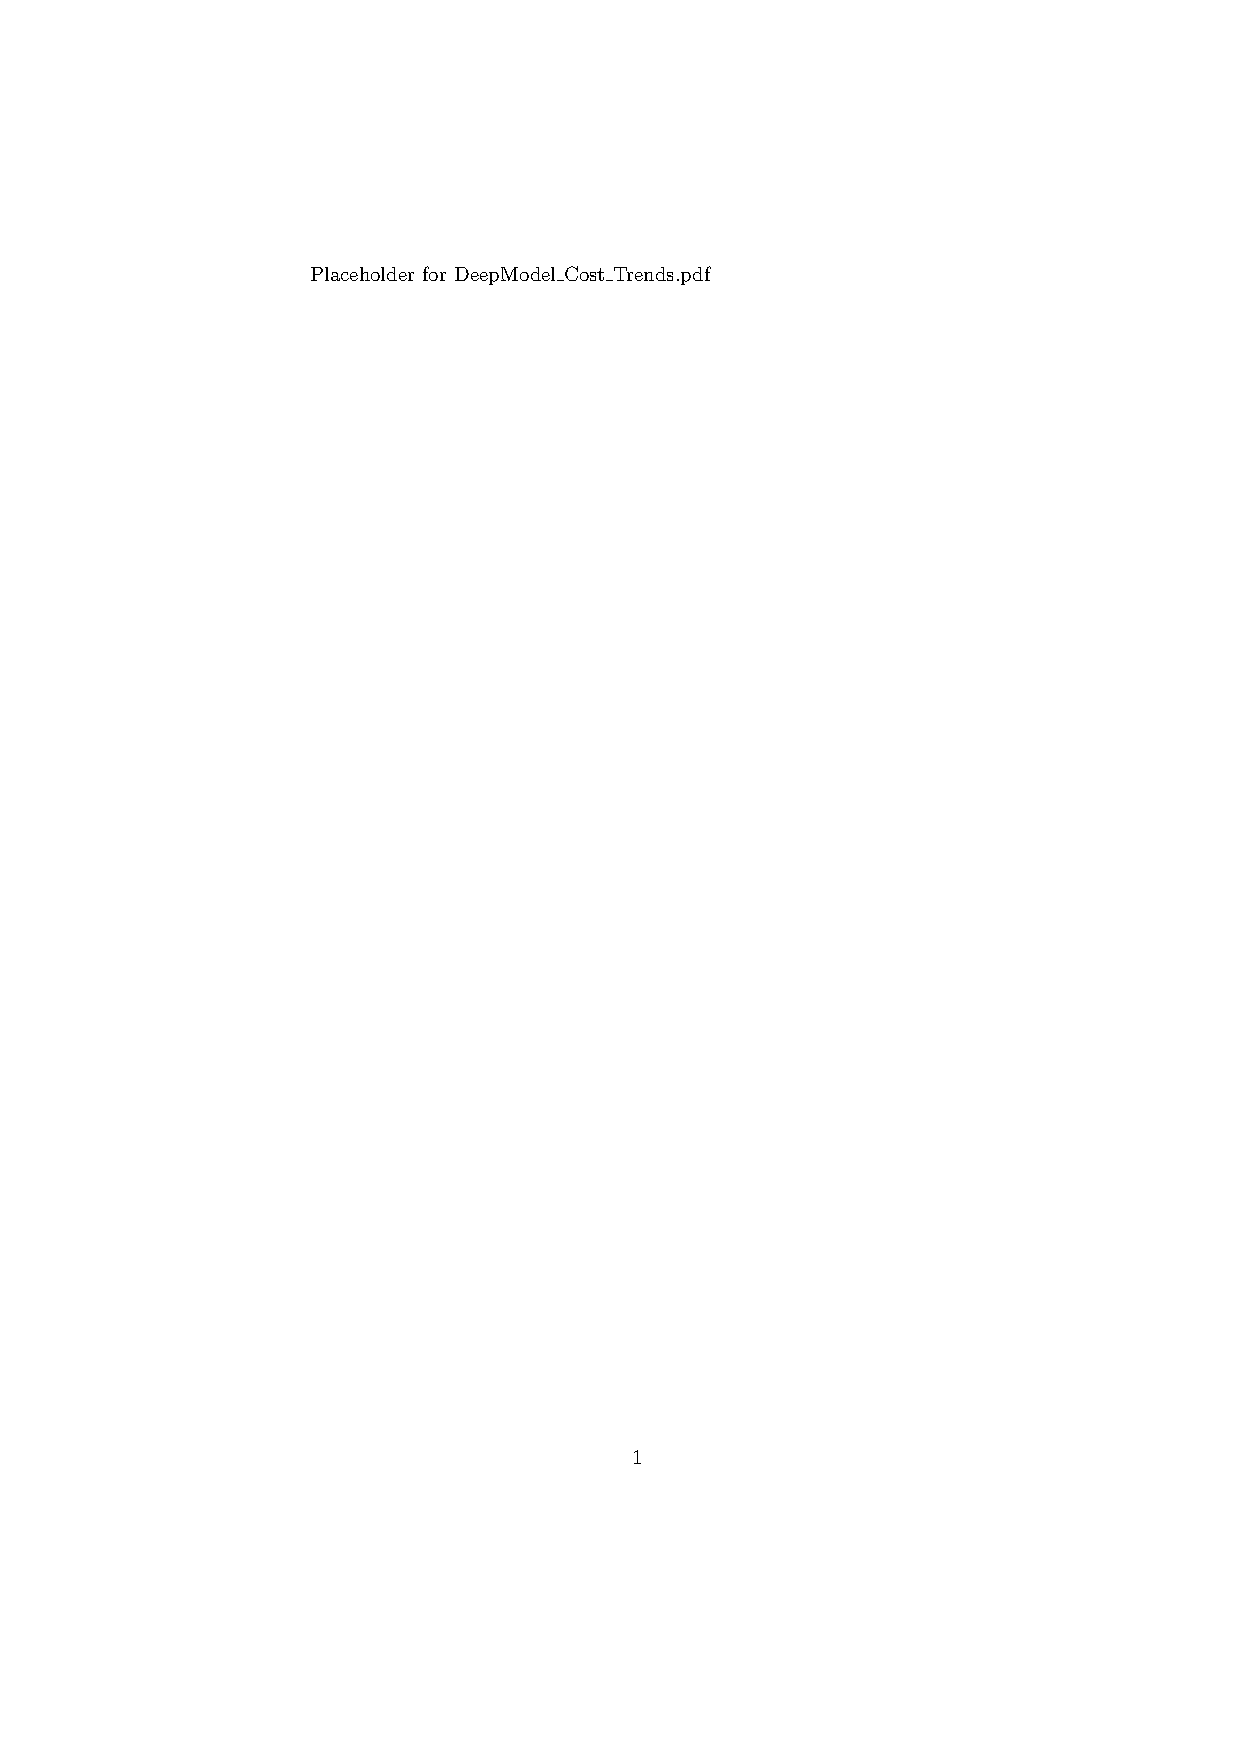
\includegraphics[width=0.8\textwidth]{DeepModel_Cost_Trends.pdf}
	\caption{深度模型规模、算力与训练成本趋势示意图}
	\label{fig:DeepModel_Cost_Trends}
\end{figure}

\section[\hspace{-2pt}国内外研究现状]{{\heiti\zihao{-3} \hspace{-8pt}国内外研究现状}}
\label{sec:intro-review}

为了应对前述挑战,研究人员从不同层面探索了多种提升深度模型构建效率的技术路径,主要可以归纳为三个方面:知识蒸馏(Knowledge Distillation)、神经架构搜索(Neural Architecture Search, NAS)与迁移,以及参数融合(Model Merging)。

\subsection[\hspace{-2pt}知识蒸馏]{{\heiti\zihao{4} \hspace{-8pt}知识蒸馏}}
知识蒸馏旨在将一个大型、复杂的“教师”模型所学习到的知识,迁移到一个轻量级的“学生”模型中,从而在保持较高性能的同时,显著降低模型的部署成本 \cite{hinton2015distilling}。
其核心思想是利用教师模型输出的“软标签”(soft targets)来指导学生模型的训练,这些软标签比传统的“硬标签”提供了更丰富的信息,揭示了类别间的相似性关系。
根据迁移的知识类型,知识蒸馏可以分为基于响应的(response-based)、基于特征的(feature-based)和基于关系的(relation-based)知识蒸馏 \cite{gou2021knowledge}。
近年来,结合提示学习(Prompt-based Learning)的少样本知识蒸馏成为研究热点,但面临着监督信号稀缺、分布偏移和教师模型输出不稳定等挑战。对比学习(Contrastive Learning)的引入,为增强学生模型在数据稀疏场景下的表示能力和噪声鲁棒性提供了新的解决思路 \cite{tian2019contrastive}。

\subsection[\hspace{-2pt}神经架构搜索与迁移]{{\heiti\zihao{4} \hspace{-8pt}神经架构搜索与迁移}}
神经架构搜索(NAS)致力于自动化设计高性能的神经网络结构,以替代耗时且依赖专家经验的人工设计过程 \cite{elsken2019neural}。
NAS方法通常包含三个核心部分:搜索空间(Search Space)、搜索策略(Search Strategy)和性能评估策略(Performance Estimation Strategy)。
尽管NAS在图像分类、目标检测等任务上取得了超越人类专家的结果,但其巨大的计算开销(通常需要数千GPU天)限制了其广泛应用。
为了解决这一问题,可迁移神经架构搜索(Transferable NAS)应运而生。其核心思想是将在一个小型代理任务上搜索到的优秀网络结构(cell)或设计原则,迁移到目标任务上,从而大幅缩减搜索成本 \cite{zoph2018learning}。
然而,当源任务和目标任务的搜索空间异构时,例如从NAS-Bench-101到NAS-Bench-201,架构的表示不兼容问题使得直接迁移变得困难。
通过对架构进行统一编码和表示学习,并学习跨空间的潜空间映射,是实现异构搜索空间之间架构迁移与重用的前沿方向 \cite{chen2021bridge}。

\subsection[\hspace{-2pt}参数融合]{{\heiti\zihao{4} \hspace{-8pt}参数融合}}
参数融合,或称模型合并(Model Merging),旨在将多个已训练好的模型参数进行融合,以低成本或“免训练”(training-free)的方式,创建一个继承了多个模型能力的单一模型 \cite{wortsman2022model_soup}。
简单的方法如权重平均(weight averaging)或模型“汤”(Model Soups),在特定场景下取得了不错的效果。
更进一步的研究,如任务向量算术(Task Arithmetic) \cite{ilharco2022task_arithmetic},通过对模型微调后产生的“任务向量”进行线性组合,实现了模型能力的灵活组合与编辑。
然而,当融合的模型数量增多或模型差异较大时,参数冲突与能力干涉(interference)问题凸显。
最近的工作,如TIES-Merging \cite{yadav2023ties_merging} 和 DARE \cite{yu2023dare},通过对任务向量进行剪枝和对齐,缓解了参数冲突问题。
如何自动地发现最优的融合“配方”,以及如何对融合过程进行更精细的控制,是该领域面临的主要挑战。

\subsection[\hspace{-2pt}研究现状评述]{{\heiti\zihao{4} \hspace{-8pt}研究现状评述}}
尽管上述三个方向都为提升模型构建效率做出了重要贡献,但目前的研究大多孤立地在各自的层次上进行,缺乏跨层次的协同与信息流动。
例如,知识蒸馏的输出(学生模型)可以作为神经架构搜索的初始种群,或者参数融合可以利用架构的相似性来指导融合策略。
此外,不同研究工作对“效率”的度量标准不一,缺乏统一的评测预算和统计口径,使得在不同方法之间进行公平比较变得困难。
本论文认为,打通知识层、结构层和参数层之间的信息壁垒,建立一个统一的、可协同优化的多层次知识迁移框架,是进一步提升深度模型构建效率的关键。

\begin{table}[htbp]
	\centering
	\caption{相关工作矩阵图}
	\label{tab:RelatedWork_Map}
	\begin{tabular}{|c|c|c|c|}
		\hline
		\textbf{层次} & \textbf{主要技术} & \textbf{代表性工作}         & \textbf{主要挑战} \\
		\hline
		知识层         & 知识蒸馏          & Hinton et al. (2015)   & 少样本、噪声、黑盒     \\
		\hline
		结构层         & NAS与迁移        & Zoph et al. (2018)     & 计算开销、异构迁移     \\
		\hline
		参数层         & 参数融合          & Wortsman et al. (2022) & 参数冲突、配方搜索     \\
		\hline
	\end{tabular}
\end{table}

\section[\hspace{-2pt}研究主线与总体思路]{{\heiti\zihao{-3} \hspace{-8pt}研究主线与总体思路}}
\label{sec:intro-outline}

本论文的核心思想是在“知识-结构-参数”三个不同层次上,系统性地研究和实践知识迁移,以应对深度模型构建的效率瓶颈。我们提出一个三层递进的研究主线,并探索各层次之间的协同优化。

\begin{itemize}
	\item \textbf{知识层迁移:} 在功能与分布层面进行迁移。我们关注于在数据稀缺的场景下,如何通过知识蒸馏,将教师模型的知识高效地迁移给学生模型。这对应于论文的第三章,我们提出了一个基于双重对比学习的少样本知识蒸馏框架Prompt-Distiller。
	\item \textbf{结构层迁移:} 在模型架构与拓扑层面进行迁移。我们研究如何将在一个任务或搜索空间上学到的优秀架构先验,迁移到新的、甚至是异构的搜索空间中,从而加速神经架构搜索的过程。这对应于论文的第四章,我们提出了一个跨异构搜索空间的进化迁移NAS方法。
	\item \textbf{参数层迁移:} 在模型权重与参数空间进行迁移。我们探索如何通过“免训练”或“弱训练”的方式,将多个预训练模型的参数进行融合,以低成本地获得一个具备多种能力的单一模型。这对应于论文的第五章,我们提出了一个基于知识图谱的多形态迁移优化参数融合框架KG-MFTO。
\end{itemize}

为了从理论上统一这三个层次的迁移,我们将它们表述为一个统一的迁移优化问题。其一般形式可以写作:
$$ \min_{\theta_s} L_t(f_{\theta_s}, D_t) + \lambda R(\theta_s; \text{先验}) $$
其中,$L_t$ 是学生模型 $f_{\theta_s}$ 在目标任务 $D_t$ 上的损失函数,$R$ 是一个正则化项,它将来自不同层次的先验知识(例如,教师模型的输出、源域的架构知识、待融合模型的参数分布等)引入到优化过程中。$\lambda$ 是权衡任务损失和迁移正则的超参数。

本论文的组织结构如下:第二章将介绍多层次知识迁移的理论基础。第三、四、五章将分别详细阐述我们在知识层、结构层和参数层所做的三个支撑性工作。第六章将对这三个层次的工作进行统一的分析,并探讨它们之间的协同优化框架。最后,第七章对全文进行总结与展望。

\begin{figure}[htbp]
	\centering
	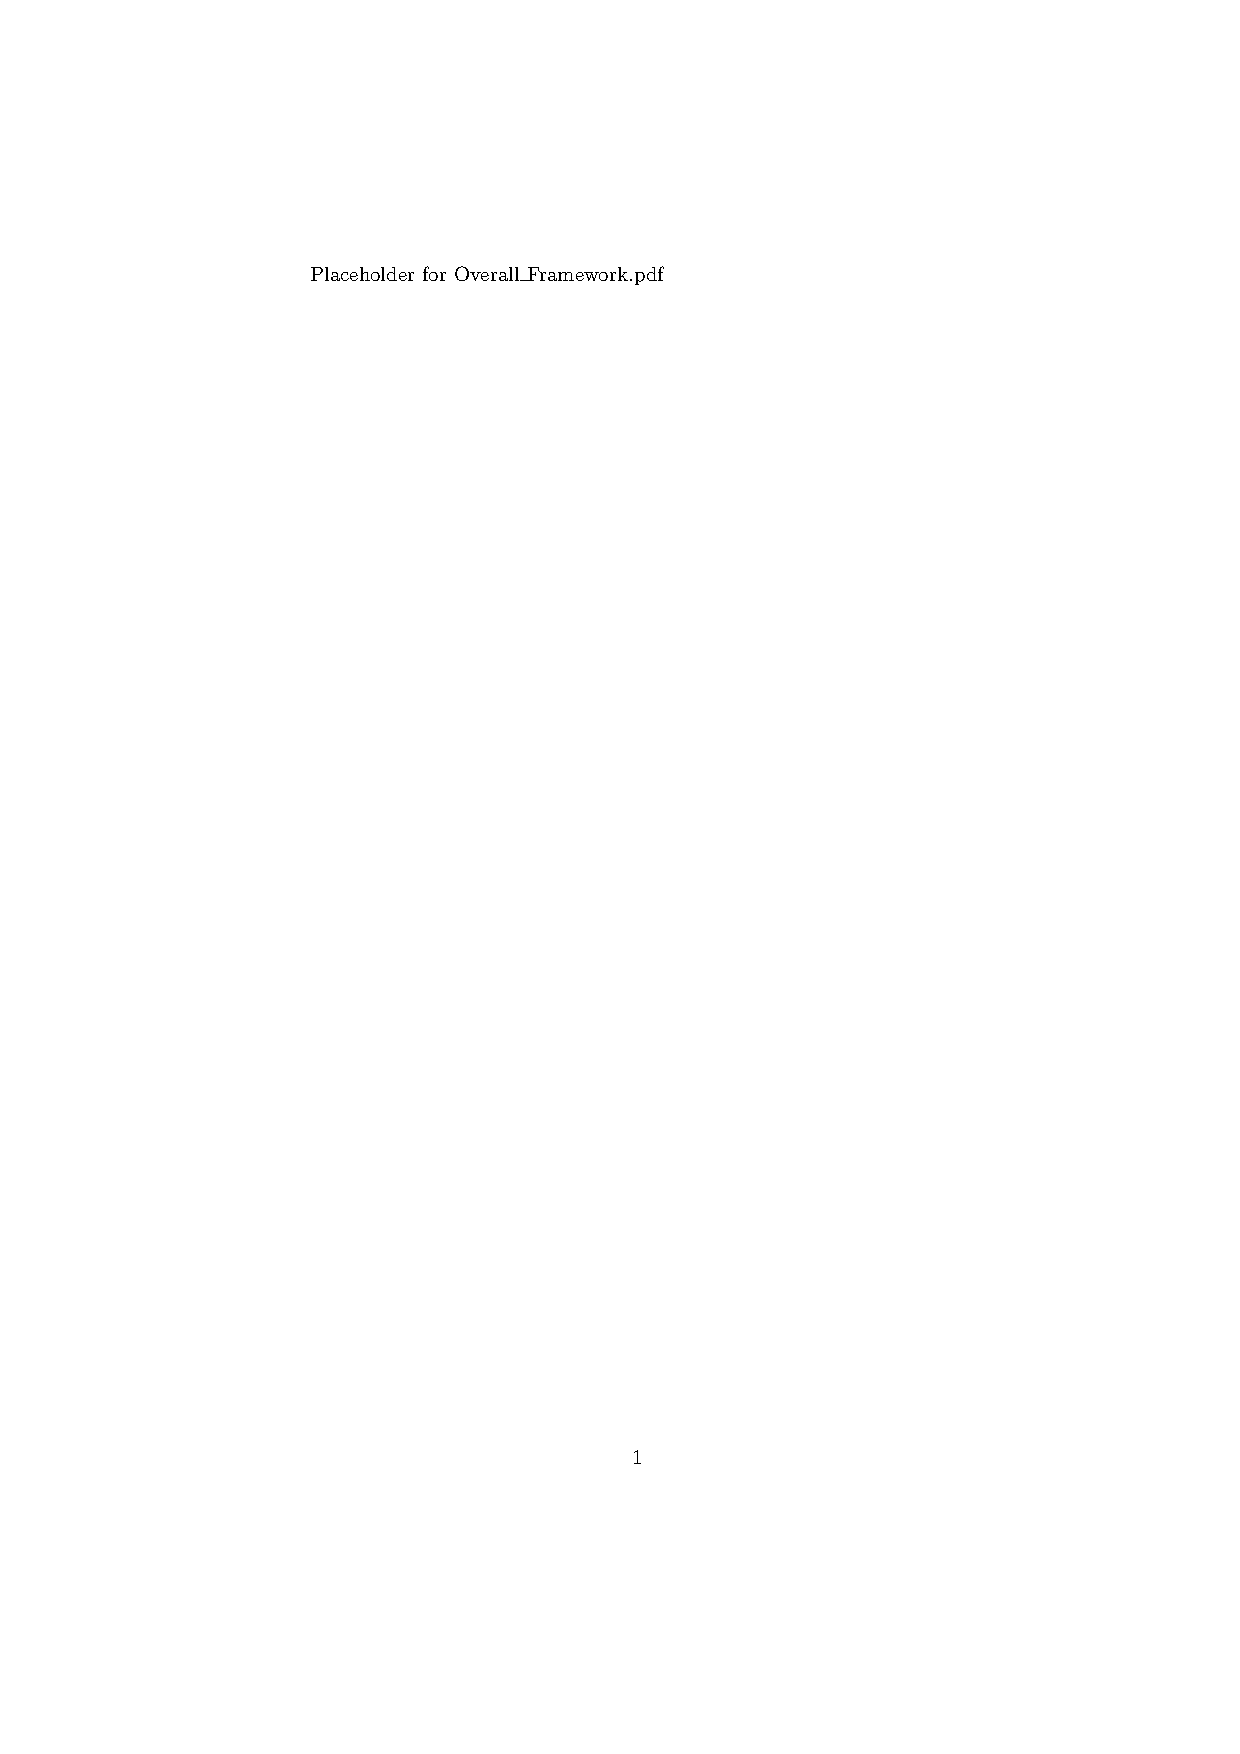
\includegraphics[width=0.8\textwidth]{Overall_Framework.pdf}
	\caption{多层次知识迁移框架与信息流示意图}
	\label{fig:Overall_Framework}
\end{figure}
